\documentclass{book}


%Packages
\usepackage{graphicx}
\usepackage[dvipsnames]{xcolor}
\usepackage{mathptmx}
\usepackage{titletoc}
\usepackage[top=2cm, left=2cm, right=2cm, bottom=2cm]{geometry}
\usepackage{fancyhdr}
\usepackage{amsmath,amsfonts,amssymb,amsthm}
\usepackage[explicit]{titlesec}
\usepackage{tikz}
\usepackage{mdframed}
\usepackage{wrapfig}
\usepackage[linktoc=all]{hyperref}
\usepackage{makeidx}
\usepackage{eso-pic}
\usepackage{xparse}
\usepackage{pgfplots}
\usepackage{paralist}
\usepackage{bm}

%Setting Images Directory
\graphicspath{{images/}}



%Defining Colors
\definecolor{pinkish}{RGB}{255, 220, 220}
\definecolor{turquoise}{RGB}{0,200,200}
\definecolor{TarletonPurple}{RGB}{79,45,127}
\definecolor{LightBlue}{RGB}{130,240,240}
\definecolor{defnGreen}{RGB}{204,255,229}
\definecolor{ocre}{RGB}{243,102,25}

\definecolor{color1}{RGB}{200, 255, 200}
\definecolor{color2}{RGB}{180, 240, 255}
\definecolor{color3}{RGB}{255, 226, 187}
\definecolor{color4}{RGB}{235, 220, 255}

\definecolor{color11}{RGB}{0, 80, 40}
\definecolor{color22}{RGB}{0, 80, 180}
\definecolor{color33}{RGB}{160, 100, 0}
\definecolor{color44}{RGB}{100, 0, 100}

%Hyper ref stuff
\setcounter{secnumdepth}{0}
\hypersetup{hidelinks,backref=true,pagebackref=true,hyperindex=true,colorlinks=false,breaklinks=true,urlcolor= black,bookmarks=true,bookmarksopen=false,pdftitle={Title},pdfauthor={Author}}


%Index Stuff

\makeindex

%Chapter Heading
\newcommand*\chapterlabel{}
\titleformat{\chapter}
 {\gdef\chapterlabel{}
  \normalfont\sffamily\Huge\bfseries}
 {\gdef\chapterlabel{\thechapter\ }}{0pt}
 {\begin{tikzpicture}[remember picture, overlay]
   \node[yshift=0cm, xshift=10.58cm] at (current page.north west)
     {\begin{tikzpicture}[remember picture, overlay]
       \node{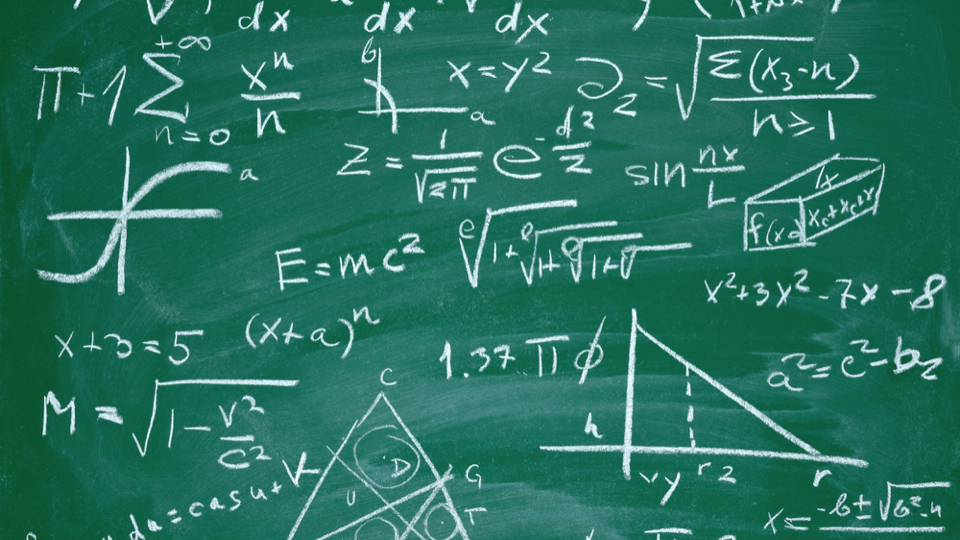
\includegraphics[width=1.1\paperwidth, height=18cm]{chalk-board-with-math.jpg}} (0,0) rectangle
         (\paperwidth,8cm);
       \draw[anchor=east] node [xshift=8cm,yshift=-7cm, rectangle,
             rounded corners=20pt,inner sep=11pt, draw=black,
             fill=white]
             {\color{black}\chapterlabel#1};
      \end{tikzpicture}
     };
  \end{tikzpicture}
 }
\titlespacing*{\chapter}{0pt}{40pt}{130pt}


%New Commands



%New Theorem Styles

\newtheoremstyle{blacknumbered}% Theorem style name
{5pt}% Space above
{5pt}% Space below
{\large\normalfont}% Body font
{0pt} % Indent amount
{\color{blue}\Large\bf}% Theorem head font
{\\}% Punctuation after theorem head
{6cm}% Space after theorem head
{}

\newtheoremstyle{thedefnone}% Theorem style name
{5pt}% Space above
{5pt}% Space below
{\large\normalfont}% Body font
{0pt} % Indent amount
{\color{color11}\Large\bf}% Theorem head font
{\\}% Punctuation after theorem head
{6cm}% Space after theorem head
{}

\newtheoremstyle{theexmplone}% Theorem style name
{5pt}% Space above
{5pt}% Space below
{\large\normalfont}% Body font
{0pt} % Indent amount
{\color{color44}\Large\bf}% Theorem head font
{\\}% Punctuation after theorem head
{6cm}% Space after theorem head
{}

\newtheoremstyle{thethmone}% Theorem style name
{5pt}% Space above
{5pt}% Space below
{\large\normalfont}% Body font
{0pt} % Indent amount
{\color{color22}\Large\bf}% Theorem head font
{\\}% Punctuation after theorem head
{6cm}% Space after theorem head
{}

\newtheoremstyle{theprblmone}% Theorem style name
{5pt}% Space above
{5pt}% Space below
{\large\normalfont}% Body font
{0pt} % Indent amount
{\color{color33}\Large\bf}% Theorem head font
{\\}% Punctuation after theorem head
{6cm}% Space after theorem head
{}

\newtheoremstyle{exercises}% Theorem style name
{5pt}% Space above
{5pt}% Space below
{\large\normalfont}% Body font
{0pt} % Indent amount
{\Large\bf}% Theorem head font
{ --}% Punctuation after theorem head
{1cm}% Space after theorem head
{}
%Frames for Environments
\newmdenv[skipabove=7pt,
skipbelow=7pt,
rightline=false,
leftline=false,
topline=false,
bottomline=false,
backgroundcolor=color1,
linecolor=red,
innerleftmargin=5pt,
innerrightmargin=5pt,
innertopmargin=5pt,
innerbottommargin=5pt,
leftmargin=0cm,
rightmargin=0cm,
linewidth=8pt]{defnbox}

\newmdenv[skipabove=7pt,
skipbelow=7pt,
rightline=false,
leftline=true,
topline=false,
bottomline=false,
linecolor=red,
innerleftmargin=5pt,
innerrightmargin=5pt,
innertopmargin=5pt,
innerbottommargin=5pt,
leftmargin=0cm,
rightmargin=0cm,
linewidth=8pt]{presentation}

\newmdenv[skipabove=7pt,
skipbelow=7pt,
rightline=false,
leftline=false,
topline=false,
bottomline=false,
backgroundcolor=color3,
linecolor=red,
innerleftmargin=5pt,
innerrightmargin=5pt,
innertopmargin=5pt,
innerbottommargin=5pt,
leftmargin=0cm,
rightmargin=0cm,
linewidth=8pt]{prblmbox}

\newmdenv[skipabove=7pt,
skipbelow=7pt,
rightline=false,
leftline=false,
topline=false,
bottomline=false,
backgroundcolor=color4,
linecolor=red,
innerleftmargin=5pt,
innerrightmargin=5pt,
innertopmargin=5pt,
innerbottommargin=5pt,
leftmargin=0cm,
rightmargin=0cm,
linewidth=8pt]{examplebox}

\newmdenv[skipabove=7pt,
skipbelow=7pt,
rightline=false,
leftline=false,
topline=false,
bottomline=false,
backgroundcolor=color2,
linecolor=red,
innerleftmargin=5pt,
innerrightmargin=5pt,
innertopmargin=5pt,
innerbottommargin=5pt,
leftmargin=0cm,
rightmargin=0cm,
linewidth=8pt]{theorembox}


%New Theorems
\theoremstyle{theprblmone}
\newtheorem{prblmx}[section]{Problem}
\theoremstyle{theexmplone}
\newtheorem{exmpl}[section]{Example}

\theoremstyle{thedefnone}
\newtheorem{defnx}[section]{Definition}
\theoremstyle{thethmone}
\newtheorem{theoremx}[section]{Theorem}
\theoremstyle{plain}
\newtheorem{theoaux}[subsection]{Theorem}
\theoremstyle{exercises}
\newtheorem{exercise}{Ex.}

%New Environments

\newenvironment{defn}
	{\begin{defnbox}
	\begin{defnx}}
	{\end{defnx}
	\end{defnbox}}


\newenvironment{prblm}
	{\begin{prblmbox}
	\begin{prblmx}}
	{\end{prblmx}
	\end{prblmbox}}	

\newenvironment{example}{\begin{examplebox}\begin{exmpl}}{\end{exmpl}\end{examplebox}}

\newenvironment{theorem}{\begin{theorembox}\begin{theoremx}}{\end{theoremx}\end{theorembox}}




	
\newenvironment{WrapBoxR}[1][r]
  {\wrapfigure{#1}{0.5\textwidth}\mdframed[backgroundcolor=LightBlue!30,skipabove=0pt,skipbelow=0pt]}
  {\endmdframed\endwrapfigure}

\newenvironment{WrapBoxL}[1][l]
  {\wrapfigure{#1}{0.5\textwidth}\mdframed[backgroundcolor=LightBlue!30,skipabove=0pt,skipbelow=0pt]}
  {\endmdframed\endwrapfigure}
  

%New Commands

\newcommand{\numline}{\begin{center}
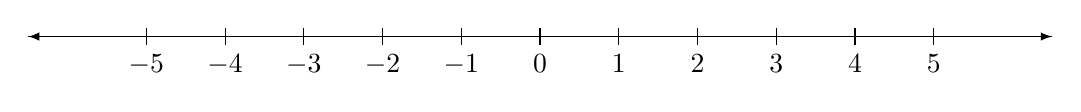
\begin{tikzpicture}
\draw[latex-] (-6.5,0) -- (6.5,0) ;
\draw[-latex] (-6.5,0) -- (6.5,0) ;
\foreach \x in  {-5,-4,-3,-2,-1,0,1,2,3,4,5}
\draw[shift={(\x,0)},color=black] (0pt,3pt) -- (0pt,-3pt);
\foreach \x in {-5,-4,-3,-2,-1,0,1,2,3,4,5 }
\draw[shift={(\x,0)},color=black] (0pt,0pt) -- (0pt,-3pt) node[below] 
{$\x$};
\end{tikzpicture}
\end{center}}

%Pgfplot stuff

\usetikzlibrary{shapes,arrows}
\usetikzlibrary{arrows.meta,positioning,calc}
\pgfplotsset{
    vasymptote/.style={before end axis/.append code={\draw[dashed,<->,-{Latex}] ({rel axis cs:0,0} -| {axis cs:#1,0}) -- ({rel axis cs:0,1} -| {axis cs:#1,0}); }},
    myaxis/.style={axis line style={<->, {Latex}-{Latex}}}
}



\begin{document}

\pagenumbering{gobble}

\thispagestyle{empty}
\pagenumbering{gobble}

\noindent
\begin{pspicture}(0,13.5)(\linewidth,0)
  \psline[linewidth=3mm,linecolor=OliveGreen](0,13.5)(\linewidth,13.5)
  \rput(\linewidth,13.5)
    {\pspolygon*(-3.6,0)(-1.4,0)(0,-1.4)(0,-3.6)}
  \rput(\linewidth,13.5)
    {\rput{-45}(-1,-1){\Large\textbf{\white Fall}}}
  \rput(\linewidth,13.5)
    {\rput{-45}(-1.5,-1.5){\Large\textbf{\white 2016}}}

  \rput[l](0,3.7){\textsl{\huge (And Some Other Functions)}}
  \psline[linewidth=3mm,linecolor=OliveGreen](0,3)(\linewidth,3)
  \psline[linewidth=3mm,linecolor=OliveGreen](0,0)(\linewidth,0)
  \rput[b](.8\linewidth,3cm)
    {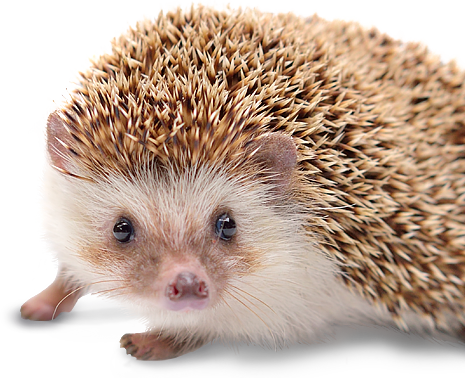
\includegraphics[height=0.3\textheight]{hedgehog.png}}
  \rput[l](0,1.5){\psscaleboxto(\textwidth,2){The Truth About Lines}}
\end{pspicture}





\chapter{How to Use This Book}

This book is an attempt to take a course such as Algebra I and treat it no differently from higher mathematical topics.  The authors feel that there is a trend in treating these lower-level concepts in a procedural fashion in stark contrast to the concept-heavy courses that mathematics majors typically encounter later in their education.  The focus here is not on exercises, but on problems in order to keep students engaged by challenging them with concepts rather than recipes.

\begin{exercise}
$2 + 9 = $
\end{exercise}

\begin{problem}
How do we add two numbers together?
\end{problem}

\begin{defn}[Solution]
A solution is any value or set of values which, when substituted for variables, makes the equation true.  A solution to an equation with multiple variables will have a value for each variable.
\end{defn}

\begin{recall}
What is the commutative property of addition?
\end{recall}

\begin{prblm}
What's something that's in the intersection of the set of flowers and the set of things that are red?
What would the intersection of the solution sets of two linear equations be like?
\end{prblm}

Other users of this 

\large
\pagenumbering{arabic}


\chapter{Operations}

Numbers come in a lot of different forms. We all know that 2 is a number. Many of us have seen $\pi$ in some capacity and recognize that it is a number. In a similar manner, you may know that $\sqrt{9001}$ and $3i + 17$ are numbers. But without understanding what these numbers mean, they are worthless. The first step in our journey towards establishing meaning for numbers starts with classification of these numbers.

\begin{boxdefn}[Number Set]
	A number set is a collection of numbers.
\end{boxdefn}

First definition down. This is a small, but significant definition as well. Number sets will be a recurring character throughout this book. 

\begin{boxdefn}[Natural Number]
	A number is called natural if we can use it to count. We denote the set of natural numbers as $\mathbb{N}$. \\ $1,2,3,4,$ and $5$ are examples natural numbers.
\end{boxdefn}

We use natural numbers every single day. However, there are some quantities that we cannot describe using natural numbers. Enter the integers.

\begin{boxdefn}[Integer]
	A number is an integer if it has no fractional part. An integer can be either positive or negative. We denote the set of integers as $\mathbb{Z}$. \\$-4, -2, 0, 3,17,  9002$ are all examples of integers. 
\end{boxdefn}


Definition overload. 


\chapter{Functions}

\begin{defn}[Function]\label{Function}
A function is the relation between a set of inputs and a set of outputs with the property that each valid input is related to exactly one output. In other words, a function takes  an input value and gives a corresponding output. We denote function $f$ evaluated for a certain $x$ as $f(x)$.
\end{defn}

You have probably seen many functions in previous math classes. Below is a visualization of a function $f$.


%function diagram

\begin{center}
\tikzstyle{decision} = [diamond, draw, fill=blue!20, 
    text width=4.5em, text badly centered, node distance=3cm, inner sep=0pt]
\tikzstyle{block} = [rectangle, draw, fill=blue!20, 
    text width=5em, text centered, rounded corners, minimum height=4em]
\tikzstyle{line} = [draw, -latex']
\tikzstyle{cloud} = [draw, ellipse,fill=red!20, node distance=3cm,
    minimum height=2em]
    
\begin{tikzpicture}[node distance = 2cm, auto]
    % Place nodes
    \node [block] (function) {$f$};
    \node [cloud, left of=function] (input) {$x$};
    \node [cloud, right of=function] (output) {$f(x)$};
    % Draw edges
    \path [line,dashed] (input) -- (function);
    \path [line,dashed] (function) -- (output);
\end{tikzpicture}
\end{center}

In this diagram, $x$ on the left is our input and the $f(x)$ on the right is the output. We can think of $f(x)$ as the function $f$ applied to $x$. Now let's look at a particular function. Let's allow the function $d$ to double any input. Now we have this diagram:

\begin{center}
\tikzstyle{decision} = [diamond, draw, fill=blue!20, 
    text width=4.5em, text badly centered, node distance=3cm, inner sep=0pt]
\tikzstyle{block} = [rectangle, draw, fill=blue!20, 
    text width=5em, text centered, rounded corners, minimum height=4em]
\tikzstyle{line} = [draw, -latex']
\tikzstyle{cloud} = [draw, ellipse,fill=red!20, node distance=3cm,
    minimum height=2em]

\begin{tikzpicture}[node distance = 2cm, auto]
    % Place nodes
    \node [block] (function) {$d$};
    \node [cloud, left of=function] (input) {$1$};
    \node [cloud, right of=function] (output) {$2$};
    % Draw edges
    \path [line,dashed] (input) -- (function);
    \path [line,dashed] (function) -- (output);
\end{tikzpicture}
\end{center}

\noindent
Our new function $d$ takes the input of 1 and gives an output of 2. In other words, the function $d$ doubled our input of 1. When a function acts on a value like this and produces an output, we write $d(1)=2$.

\begin{presentation}
	\begin{defn}[Domain]\label{Domain}
		The domain of a function is the set of all possible inputs that give valid outputs for the function.
	\end{defn}
\end{presentation}

The domain of a function is just a fancy way of saying anything we can put into the function and have the function still work. Consider a paper shredder. If we were to consider this a function, the domain would be paper, credit cards, and late homework. 
\begin{defn}[Range]\label{Range}
	The range of a function is the set of all possible outputs for that function.
\end{defn}

Let's think back to the paper shredder. If the domain of the paper shredder function was paper, credit cards, and late homework, what would be in the range? In other words, what are our possible outputs? In the case of the paper shredder, finding the domain and range are fairly easy since the paper shredder turns all inputs into shredded versions of themselves. However, most of the time this semester, we will be dealing with mathematical functions that have some effect on numerical inputs. The doubling function $d$ is a classic example of this. 

\begin{prblm}[Expressing a function as an equation]\label{Doubling Function}
Using the definition of an equation and your knowledge of the doubling function discussed above, express the function $d$ as an equation. \vspace{4cm}
\end{prblm}

Expressing a function as an equation is going to be the most common way that we look at functions this semester, but not the only way. Sometimes it may be easier to look at and analyze a function using a table of values. 

\begin{presentation}
\begin{example}[Expressing a function using a table of values]\label{Table of Values}
	Think back to the paper shredder function. If wanted to express this function using a table of values, it would like like the following.
\begin{center}
\textbf{Paper Shredder Function} \\
\begin{tabular}{|c|c|c|c|}
\hline
\textbf{input} & paper & credit card & late homework \\
\hline
\textbf{output} & shredded paper & shredded plastic & lower grade \\	
\hline
\end{tabular}
\end{center}

\noindent
 These tables of values become even more useful when dealing with a function that has numerical values. Consider the doubling function $d$.

\begin{center}

\textbf{The Doubling Function} \\
$
\begin{array}{|c|c|c|c|c|c|}
 \hline
 \bm{x} & 1 & 2 & 3 & 4 & 5 \\
 \hline
 \bm{d(x)} & 2 & 4 & 6 & 8 & 10 \\
 \hline
\end{array}
$
\end{center}

\noindent
In some situations, this is the only format in which a function is given to us. Therefore, both reading accurately and creating these tables are important tools for moving forward with functions. 
\end{example}
\end{presentation}

The last major format that functions come in is graphically. 

\pagebreak 

\begin{presentation}
\begin{defn}[Cartesian Plane]\label{The Cartesian Plane}
	The Cartesian Plane is a plane (meaning it's flat) made up of an \color{blue}$x$-axis (the horizontal line) \color{black} and a \color{red} $y$-axis (the vertical line). \color{black}
	\begin{center}
%	\begin{tikzpicture}
%	\begin{axis}[axis background/.style={fill=white}, width=12cm, ymax=10, ymin=-10, xmax=10, xmin=-10, axis lines=middle, grid=major, myaxis, xticklabel style= {font=\tiny, yshift=0.5ex}, yticklabel style={font=\tiny, xshift=0.5ex},xtick={-10,...,10}, ytick={-10,...,10}	]
%	\end{axis}
%	\end{tikzpicture}
	\end{center}
Points on the Cartesian plane are labeled using an $x$-$y$ coordinate. The notation for these coordinates is $(x,y)$. For example, the point with an $x$-value of -4 and a $y$-value of 3 is $(-4,3)$. The point at which the $x$ and $y$ axis meet is called the origin and has an $x$ and $y$ value of 0, giving it the notation $(0,0)$. 

\smallskip
We say that the Cartesian Plane has 4 separate parts, which we call the 4 Quadrants, and are separated by the $x$ and $y$ axes. The first Quadrant is when we have both positive $x$ and $y$ values, which is in the top right corner of the plotted axes above. By moving counterclockwise from the top right, we cross through the second, third, and fourth quadrants in that order. 
\end{defn}
\end{presentation}

\begin{prblm}[Graphing the doubling function]
Let's practice graphing functions by graphing our doubling function $d$, which we already have an equation for (\ref{Doubling Function}).
\vspace{5cm}
\end{prblm}

\begin{presentation}
\begin{example}[Expressing a function using a graph]
Sometimes functions are expressed on the Cartesian Plane. We can use these representation to gather the same information we can get from the others. 
\begin{center}
\begin{tikzpicture}
	\begin{axis}
	%[axis background/.style={fill=white},width=12cm,ymax=10,ymin=-10,xmax=10,xmin=-10,axis lines=middle,grid=major,myaxis,xticklabel style={font=\tiny,yshift=0.5ex},yticklabel style={font=\tiny,xshift=0.5ex},xtick={-10,...,10},ytick={-10,...,10}]
	%	\begin{axis}[axis background/.style={fill=white}, width=12cm, ymax=10, ymin=-10, xmax=10, xmin=-10, axis lines=middle, grid=major, myaxis, xticklabel style= {font=\tiny, yshift=0.5ex}, yticklabel style={font=\tiny, xshift=0.5ex},xtick={-10,...,10}, ytick={-10,...,10}]
	\addplot+[smooth] coordinates {(-2,-8) (-1,-1) (0,0) (1,1) (2,8)};
	%\addplot+[smooth] coordinates {(-2,-8) (-1,-1) (0,0) (1,1) (2,8)};
	\end{axis}
\end{tikzpicture}
\end{center}


This function is the cubic $(x^3)$ function, restricted to the domain -2 to 2. 


\end{example}
\end{presentation}

\begin{presentation}
\begin{defn}[Intercepts]\label{Intercept}
	An intercept of a function is a point where the function crosses (or intercepts) any axes. A function can have multiple intercepts.
\end{defn}
\end{presentation}

When talking about intercepts, we usually distinguish between the $x$-intercepts and the $y$-intercept.

\begin{prblm}
What must be the $y$ coordinate of a $x$-intercept? How do we know this? What must be the $x$ coordinate for the $y$-intercept?	
\vspace{4cm}
\end{prblm}

\newpage
\begin{prblm}

Consider the following function:
\begin{center}
\begin{tikzpicture}
	\begin{axis}
	%[axis background/.style={fill=white}, width=12cm, ymax=10, ymin=-10, xmax=10, xmin=-10, axis lines=middle, smooth, grid, myaxis, xticklabel style= {font=\tiny, yshift=0.5ex}, yticklabel style={font=\tiny, xshift=0.5ex},xtick={-10,...,10}, ytick={-10,...,10}]
	\addplot[color=red] coordinates {(-9,0) (-8, 1) (-4, 6) (-2, 4) (0, 5) ( 2, 3) (4, 0) (5, -2) (8, -6)};	
	\addplot[mark=*, color=red] coordinates {(-9,0)};
	\addplot[mark=*, color=red] coordinates {(8, -6)};
	\end{axis}
\end{tikzpicture}
\end{center}

\noindent
What is the domain of this function? What about the range? What are the intercepts of the function?
\vspace{4cm}
\end{prblm}


\pagebreak


\section*{Exercises}

\begin{exercise}
For the following functions, find $f(3)$:

\begin{itemize}
\item $f(t) = 4t$
\item $f(t) = -\frac{1}{2}t + 1$
\item $f(x) = x^2 - 2x + 1$
\item $f(x) = 2$
\item $f(z) = 7$
\item $f(z) = z^3-z^2-z-1$
\end{itemize}

\end{exercise}
\bigskip

\begin{exercise}
Build a table for the following functions:

\begin{itemize}
\item $f(t) = t + t + t + t + t$
\item $f(x) = 1-x^{2}$
\item $f(q) = q^{120}\times 0$
\end{itemize}

\end{exercise}
\bigskip

\begin{exercise}
If $f(x) = x^2$, find $x$ where $f(x) = 4$.
\end{exercise}
\bigskip

\begin{exercise}

Given $f(x) = 3x + 20$
	\begin{multicols}{2}
		Evaluate:
		\begin{itemize}
		\item $f(-5)$
		\item $f(0)$
		\item $f(1)$
		\item $f(9001)$
	\end{itemize}
	\columnbreak
		

		Find $x$ such that:
		\begin{itemize}
		\item $f(x)=-5$
		\item $f(x)=0$
		\item $f(x)=1$
		\item $f(x)=9001$
	\end{itemize}
\end{multicols}

\end{exercise}

\bigskip

\begin{exercise}
Make a table with a column for each of the following functions, making sure to include some negative values:

\begin{itemize}
\item $f(x) = x$
\item $g(x) = x^2$
\item $h(x) = x^3$
\item $j(x) = x^4$
\end{itemize}

Describe the difference between the functions based on this table.

\end{exercise}
\bigskip

\pagebreak

\begin{exercise}

Let 
\begin{itemize}
\item $f(x) = \frac{2}{5}x$
\item $g(x) = 2 - 3x$
\end{itemize}

\noindent
Find $f(10)$, and then put that value into $g(x)$.  Then, find $g(10)$, and put that value into $f(x)$.  Compare these values.

\end{exercise}

\bigskip
\begin{exercise}
	Create two tables with different scales for the function $f(x) = x^2 - 9$.
\end{exercise}
\bigskip

\begin{exercise}
The following is a table of two functions

\begin{center}
\begin{tabular}{|c|c|c|}
\hline
$x$ & $f(x)$ & $g(x)$ \\
\hline
-2 & -50 & 1\\
\hline
-1 & -2 & 3\\
\hline
0 & 14 & 10\\
\hline
1 & 16 & 3\\
\hline
2 & 15 & 1\\
\hline
\end{tabular}
\end{center}

What is $g(x)$ when $f(x) = -2$?

For which values of $x$ is $f(x) > g(x)$?

\end{exercise}
\bigskip

\begin{exercise}

Toaster function:

In the domain of the toaster function, we have bread, pop-tarts, and bagels, as we expect.  We also could put toast back into the toaster function, as well as the resulting charcoal.  The table would look like the following:

\begin{center}
\begin{tabular}{|c|c|}
\hline
$x$ & toaster$(x)$\\
\hline
bread & toast\\
\hline
pop-tart & pop-tart\\
\hline
toast & charcoal\\
\hline
charcoal & ashes\\
\hline
bagel & bagel\\
\hline
\end{tabular}
\end{center}

What is $a$ if toaster$(a) = $ charcoal?

What is $a$ if toaster$($charcoal$)$ $ = a$?

Explain.

\end{exercise}
\bigskip

\begin{exercise}
Give three functions for which $f(5) = 0$
\end{exercise}
\bigskip

\begin{exercise}
Some sort of respiratory illness has infected some of a farmer's cattle.  He has decided to use amoxicillin to treat them.  The dosage guidelines of amoxicillin are 2 milliliters for every 100 pounds the animal weighs.  Create a table and a graph which show the relationship between the weight of an infected cow and the amount of antibiotic needed to treat it.
\end{exercise}


\pagebreak

\begin{exercise}
While the sun never sets on the British empire, its control has changed appreciably over the years.  The following is a chart of the land area of the British Empire for various years.\footnote{https://en.wikipedia.org/wiki/Territorial\_evolution\_of\_the\_British\_Empire\#/media/File:Riseandfall1.PNG}

\begin{center}
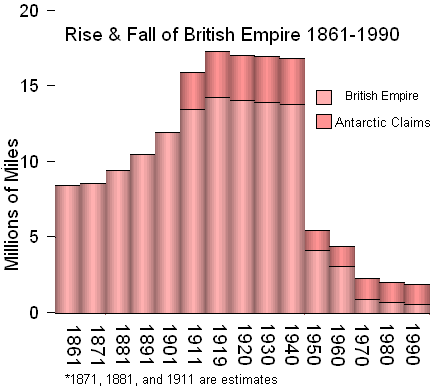
\includegraphics{images/Riseandfall1.png}
\end{center}



In what time interval is the territory of the British Empire growing?  In what time interval is it shrinking?  Let $f(t)$ be the function of land area of the British Empire over time, where $t$ is the current year.  Estimate $f(1940)$ and $f(1950)$.  Find $t$ where $f(t)$ is the highest.

\end{exercise}
\bigskip

\begin{exercise}
Liam weighs 205 pounds and is looking to put on another 10 pounds in muscle over the next 6 months.  He lifts three days per week, and his trends in the past have been to stay at the same weight with a 30-minute workout.  His gain after 6 months is usually one pound for each additional 5 minutes he works out for each session.

How long should he plan to lift each session to meet his goal?
If he plans to lift for 60 minutes each session, how much should he expect to gain in 6 months?
\end{exercise}
\bigskip

\begin{exercise}
Before the beginning of each school year, you, a teacher, need to order enough books for your students, plus a few backup copies.  There are 4 books they each need, and you want 5 replacements for each book, regardless of how many students you have.  Give an equation, table, and graph for this relationship.
\end{exercise}


\pagebreak
\begin{exercise}
To set up your account with the electric company, you must pay a \$90 activation fee.  Your plan is 10 cents per kilowatt-hour.  Additionally, based on information from previous accounts, they have determined that your average bill over the year is \$70.  How much money will you give the electric company this year?  Create a table for the amount you've given the electric company as a function of time.
\end{exercise}



\begin{exercise}
You're considering subscribing to Netflix.  You don't watch very many TV shows, but you watch movies occasionally.  The main competitor for your purposes is Redbox, which rents individual movies for \$1 each.  Netflix is for \$10 each month.

Make a table of the per-month price for each Netflix and Redbox, based on the number of movies you watch each month.  How could this table influence your decision?

\end{exercise}

\begin{exercise}
A local community can estimate their corn yield per acre by keeping track of the greatest number of consecutive days without rain.  They estimate 180 bushels as a high mark, but subtract the greatest number of consecutive days without rain.

How many consecutive days without rain would the community have to have before they estimate only 140 bushels per acre?
\end{exercise}
\bigskip

\begin{exercise}
	The $3^{\prime\prime}$ cactus in my window grows at a rate of $\frac{1}{4}^{\prime\prime}$ per month.  Give an equation, table, and graph which express its height over time.
\end{exercise}
\bigskip

\begin{exercise}

The amount of gas required to start a certain engine is 8 milliliters.  This engine also consumes 0.4 milliliters of gas every second it spends idling.  Create an equation, table, and graph to express this relationship.

\end{exercise}
\bigskip

\begin{exercise}
If a baseball (or, really, any other object) is thrown upward at 40 meters per second, the following equation describes its height as a function of time:

$$f(t) = 2 + 40t - \frac{1}{2}9.8t^2$$

Create a table and a graph for the function.  Make sure to include values of $t$ from 0 to 10.  Using as few math terms as possible, describe what this function is telling us.

\end{exercise}
\bigskip








\chapter{Linear Functions}

Now that we have a good understanding of what a function is, it's time to begin exploring one of the most common types of functions: the linear function.


\begin{defn}[Linear Function]\label{Line}
	A linear function is a function that increases at a constant rate. The \hyperref[Solution Set]{solution set} of a linear function is an infinite number of points. 
\end{defn}


\section{Slope-Intercept Form}

When the equation of a linear function takes the form
\begin{equation}
f(x) = mx + b
\end{equation}

\noindent
we say it is in slope-intercept form.  When we're looking at equivalent equations, this form is one of the most useful for plotting the line, because when we choose a value for $x$, the right side of the equation turns into an expression that we can simplify to find $f(x)$.  This form of an equation also contains useful information that we can use to make plotting lines faster.  The $m$ is the slope.  The $b$ is the vertical-intercept. 

Notice that $y$ is not being included in this formula. There is a reason for that. We want to think about these lines as representations of functions. Therefore, throughout this chapter, the vertical axis will sometimes be referred to as the $f(x)$ axis and the coordinates will sometimes be referred to as an $x$ coordinate and a $f(x)$ coordinate (in the form $(x, f(x))$. This works the same as you might be used to, but with this notation, we have more flexibility with what variables we use. Whether we use the variable $y$ or the function notation $f(x)$, we are talking about the output of a function. 

	
\begin{defn}[Slope]
	The slope of a line is a number representing how steep the line is. It is calculated by finding the rate of change of the function. The higher the value of the slope, the steeper the line is. A negative slope indicates that, as the x-value increases, the line slants downward.
\end{defn}

The rate of change is a central idea to understanding functions. For functions in general, we find the average rate of change by looking at the change in output and dividing that by the change in input.
\[
\text{Average Rate of Change}=\frac{\triangle \text{output}}{\triangle \text{input}}
\]

\noindent
But when we are dealing with lines, the rate of change is always constant. So instead of finding the average rate of change, we can find the exact rate of change. 

\begin{example}[Finding the Slope from a Graph]\label{Slope on a graph}
	\begin{center}
	\begin{tikzpicture}
	\begin{axis}		%Uncommenting the following line and putting it on this line with no space results in an error.
	%[axis background/.style={fill=white}, width=12cm, ymax=10, ymin=-10, xmax=10, xmin=-10, axis lines=middle, grid=major, myaxis, xticklabel style= {font=\tiny, yshift=0.5ex}, yticklabel style={font=\tiny, xshift=0.5ex},xtick={-10,...,10}, ytick={-10,...,10}]
	\addplot+[smooth] coordinates {(-9,-8) (9,5)};
	\end{axis}
\end{tikzpicture}
	\end{center}
	
Here we have a linear function, graphed on the domain of $[-9,9]$. If we are asked to find the slope(or rate of change) of this function, we have all the information we need on the graph. If the rate of change is $\frac{\triangle\text{output}}{\triangle\text{input}}$, then how would we find our slope?
\end{example}


Unfortunately, we don't always have a beautiful picture to look at to find the slope.  Sometimes, we only have some points that we can use.  However, if we're told that these points are on a linear function, we can use the same kind of reasoning to find the slope.  Since each point has an $x$ and a $f(x)$ value, we'll use those in what we call the slope formula.

It's valuable to remember that order is important.  If Angelica has 3 cookies today, and 2 cookies tomorrow, the change in cookies is 1, but when we're talking about lines, we need to know if the number went up one or down one.  We find differences by subtracting, so we need to make sure we choose the right order for subtracting one value from the other.  Here, we would want to subtract the value of today from the value of tomorrow, to make sure we have a negative number, to show that the number went down by one.

The same applies to points.  When we want to find the change in $x$, we want to be careful to choose which point is first and which one is second.  It won't matter which is which as long as you keep the $x$ and $f(x)$ values together.

\begin{equation}
m = \frac{f(x_2) - f(x_1)}{x_2 - x_1}
\end{equation}

\begin{example}

If we have two points, (2,3) and (5,6), we want to choose one point to be first.  Let's have (2,3) be first.  Each point has an $x$ and a $f(x)$ value, so the first point's $x$-value is 2.  We call this value $x_1$ in the formula.  The second points $x$-value is 5, and we call it $x_2$.  This pattern gives us everything we need to plug into the formula.  However, we need to be careful to use to the same order when we use the $f(x)$-values.  $f(x_1)$ is 3, and $f(x_2)$ is 6.  When we plug these in, $$m = \frac{6 - 3}{5 - 2}$$

We can then simplify this to $\frac{3}{3}$, which simplifies further to 1.  This tells us that the line that these points come from has a slope of 1.
\end{example}



\section{Point-Slope Form}

As we've learned previously, for any equation, there are countless equivalent equations.  In addition to having a slope-intercept form, equations also have a point-slope form.  If equations in slope-intercept form use the valuable information of slope and intercept, what kinds of information can we get from a line in point-slope form?

The point-slope form of a line looks like the following.

\begin{equation}
y - k = m(x-h)
\end{equation}

In this form, m is still the slope, but we have two new values, h and k.  These are the x and y values of a point on the line, (h,k).  This form of a line is sometimes useful to find, but more often it is used as a formula to plug values into.  As its name suggests, if you have the slope of a line and a point on it, you can find the equation of the line.

\begin{example}
If a line has slope 1 and passes through the point (2,3), what is the equation of the line in slope-intercept form?

We take the information we are given and understand that, with the point and the slope, we use the point-slope form of the line, and we can plug those values straight in.

The point (2,3) is our point (h,k) from the form of the line.  So we take the equation $y - k = m(x - h)$ and plug them in, to get $y - 3 = m(x - 2)$.  We also take the slope, 1, and plug it in for m to get $y - 3 = 1(x - 2)$.  Now the we have no variables other than x and y, we can solve for y. to get the slope-intercept form.

$y - 3 = x - 2$

$y = x + 1$

\end{example}

With all of the information we have so far, we can find the y-intercept, slope, equation, and any points we need from a graph of a line.  We can also find the y-intercept, slope, equation, and graph from only two points on the line.  The most valuable skill for learning this is the concept of equivalent equations.












 
\begin{example}
The tables below are input/output tables for the function $f(x)=2x+1$. Notice that they contain the same information and are just oriented differently.
\begin{center}
\begin{tabular}{|c|c|}
\hline
	x & f(x) \\
	\hline
	1 & 3 \\ 
	\hline
	2 & 5 \\
	\hline
	3 & 7 \\ 
	\hline
	4 & 9 \\
	\hline 
\end{tabular}	\hspace{3cm} \begin{tabular}{|c|c|c|c|c|}
\hline
	x & 1&2 & 3 & 4 \\
	\hline
	f(x) & 3 & 5 & 7 & 9 \\
	\hline
\end{tabular}
\end{center}

Fun fact: the ordered pairs given to us from these tables make up coordinates on the Cartesian Plane. Therefore, we have the four coordinates (1,3), (2,5), (3,7), and (4,9) for the function $f(x)=2x+1$. 
\end{example}


\begin{example}

Sometimes we are given a table and asked questions about it. For example: Can we tell if the function $f(x)$ is linear, given the table below?
\begin{center}
\begin{tabular}{|c|c|}
\hline
	x & f(x) \\
	\hline
	5 & 17 \\ 
	\hline
	6 & 20 \\
	\hline
	7 & 21 \\ 
	\hline
	8 & 23 \\
	\hline 
\end{tabular}
\end{center}

The answer is no. We can see that the inputs do increase at a constant rate (1), but the outputs do not increase at a constant rate. Therefore, the function cannot be linear.
\end{example}

\begin{prblm}
	If we assume that the function $g(x)$ is linear, can we fill in the input/output table?
	
		\begin{center}
	 \begin{tabular}{|c|c|c|c|c|}
\hline
	x & 1&2 &  &  \hspace{.5cm} \\
	\hline
	g(x) & 4 &  & 12 &  \\
	\hline
\end{tabular}
\end{center}

\end{prblm}
	
\section{Intersections as a Concept}

An important idea in math is the idea of a set.  Sets are collections of objects.  We can talk about the set of flowers, the set of things that are red, or whatever other category of thing we can think of.  If something belongs to both sets, we say that it is in the intersection of those sets.


\begin{prblm}
What's something that's in the intersection of the set of flowers and the set of things that are red?
What would the intersection of the solution sets of two linear equations be like?
\vspace{5cm}
\end{prblm}


We've briefly mentioned sets before.

Recall: What is the solution set for the line $y=-x$? What about the line $y=2x+1$?


\begin{defn}[Linear System]
A linear system is made up of multiple linear equations. The solution set for a linear system is the intersection of the solution sets of the linear functions. 
\end{defn}

Over the course of the past few sections, we've been reinforcing this idea that plotting a linear equation as a line makes some features easier to see, such as other solutions, and overall trends of those solutions.  Furthermore, finding the equation that goes with a line that has been plotted gives us some extra power, such as the ability to find solutions that are outside of the plot, or express the facts of the situation in words so that we can communicate these ideas more easily.

\begin{defn}[Consistent System]
We call a linear system consistent if and only if there exists a solution.	
\end{defn}

\begin{prblm}
Find some solutions to the equation $y = 3 - x$.
Find some solutions to the equation $y = 2x$.

How would you find the intersection of their solution sets?

\vspace{5.5cm}
\end{prblm}

However, there are some lines that do not intersect.

\begin{defn}[Parallel Lines]
We call two lines with the same slope parallel lines. If two lines are parallel, they will never intersect. Likewise, if two lines intersect, then they are not parallel. 	
\end{defn}
This is an important definition to remember, especially when we are dealing with graphing two separate lines on the same graph.

\begin{defn}[Inconsistent System]
We call a linear system inconsistent when there is no point of intersection (no solution).	
\end{defn}

\begin{theorem}[Solutions of a Linear System]
There is either a single solution, no solution, or infinite solutions to a linear system with two equations. 	
\end{theorem}

\noindent
\textbf{\underline{Evidence}:} Consider the possibilities for two lines in a linear system. The first case is they intersect. To see an example, flip back to Example 1.4. Since lines remain straight, they will never intersect again. There is our first case (a single solution). If they don't intersect, then Definition 1.6 tells us that they must be parallel. In most cases, if two lines are parallel, then the system will have no solution, since there is no point in which they will intersect, confirming our second case (no solution). Finally, there is one particular case that we have not mentioned yet. If two lines are equivalent, then the solution set will be infinitely large, since every point will intersect, which gives us our last result (infinite solutions). Thus, the theorem is true. 
\pagebreak

\section{Graphing Linear Systems}

We've mentioned before that a coordinate system can be created with any scale we want.  The $x$ and $y$ axes don't even need to have the same scale.  That idea requires some refinement now: if we put two lines on the same coordinate system, we have to use them same scale for each line.  When we do this, if we're plotting the line from a set of points, we need to make sure we finish plotting the first line before moving on to the second.

%Insert Illustration

\begin{figure}[ht] 
  \label{ fig7} 
  \begin{minipage}[b]{0.5\linewidth}
    \centering
    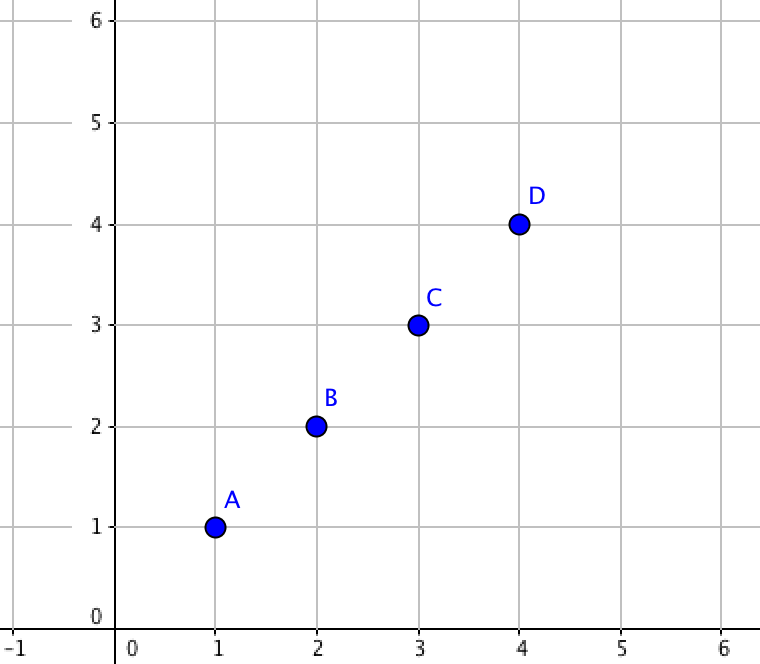
\includegraphics[width=.5\linewidth]{points.png} 
    \caption{Plotting points for the line $y=x$.} 
    \vspace{4ex}
  \end{minipage}%%
  \begin{minipage}[b]{0.5\linewidth}
    \centering
    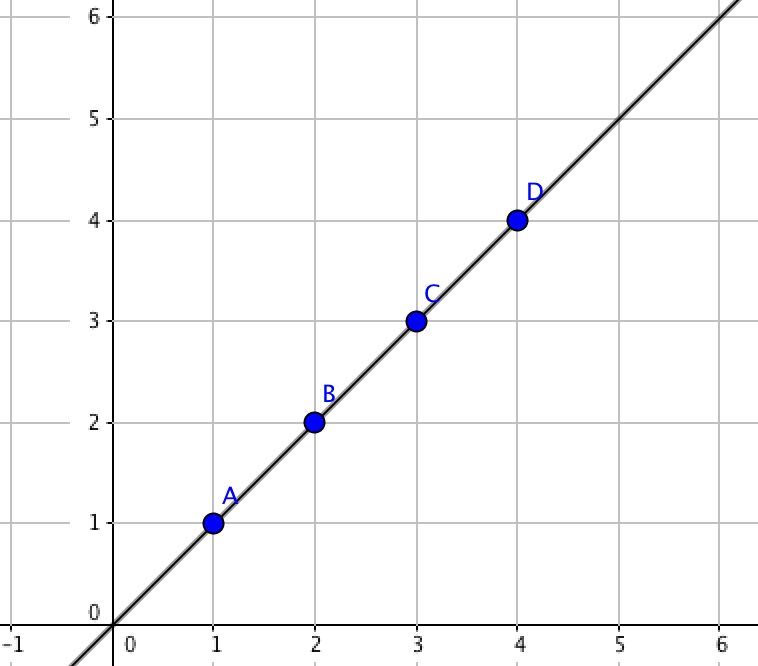
\includegraphics[width=.5\linewidth]{pointsline.png} 
    \caption{The line $y=x$.} 
    \vspace{4ex}
  \end{minipage} 
  \begin{minipage}[b]{0.5\linewidth}
    \centering
    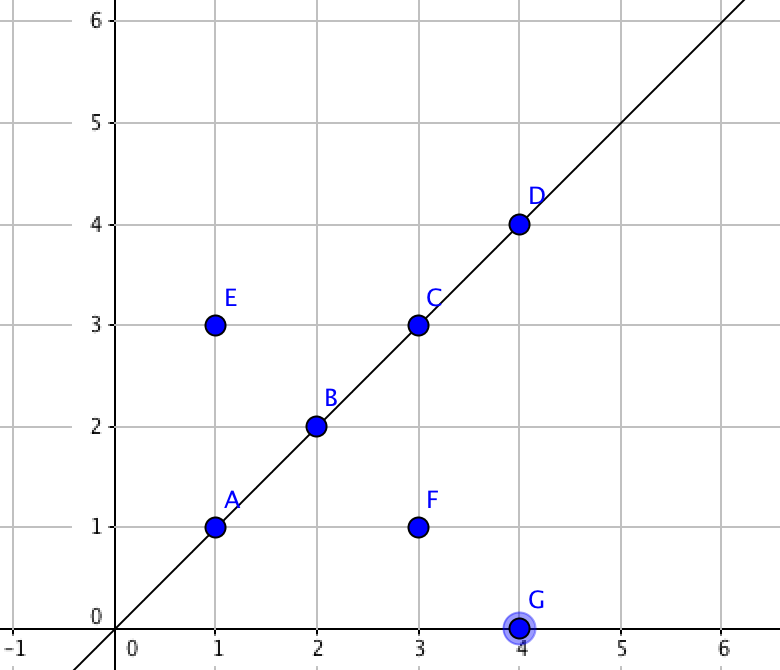
\includegraphics[width=.5\linewidth]{points2.png} 
    \caption{Plotting points for a new line.} 
    \vspace{4ex}
  \end{minipage}%% 
  \begin{minipage}[b]{0.5\linewidth}
    \centering
    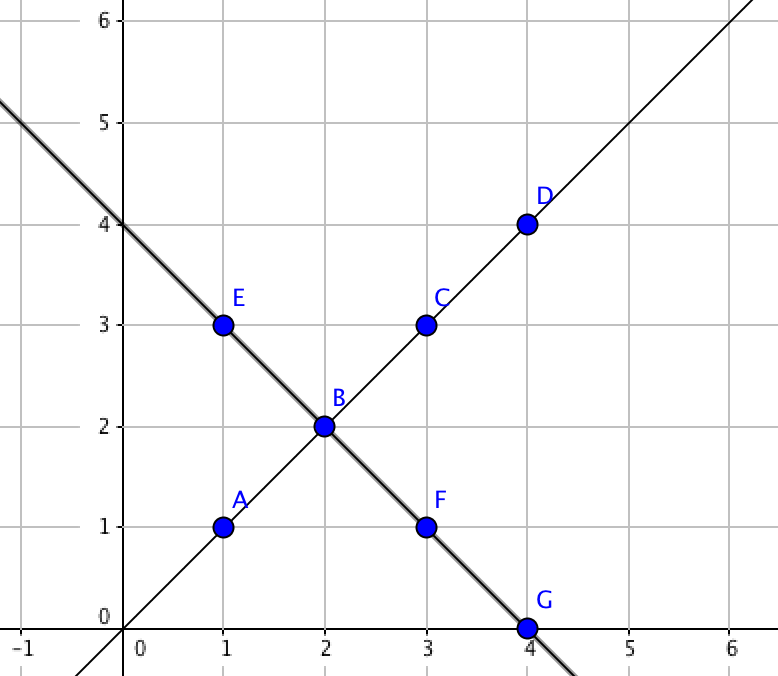
\includegraphics[width=.5\linewidth]{line2.png} 
    \caption{The lines $y=x$ and $y=-x+4$.} 
    \vspace{4ex}
  \end{minipage} 
\end{figure}


It's no coincidence that we call the objects in two sets the ``intersection''.  A single solution in the solution set of an equation is a point on the line that corresponds to that equation.  If we have two lines on a graph, the point where they intersect is a point that's on both of the lines at the same time.  That means that the point is going to be in the solution set of both equations.

\begin{example}
Find the intersection for the following system of linear equations.
$$y - 4x = -4$$
$$2y + x = 10$$

Using this strategy, we want to plot both equations.  To do this, we want them in a form that we can use to plot them, so we'll put them in slope-intercept form.
For the first line:
$$
\begin{array}{rcl}
y - 4x & = & -4 \\
y & = & 4x - 4 \end{array}$$

And for the second line:
$$\begin{array}{rcl}
2y + x & = & 10 \\
2y & = & 10 - x \\ 
y & = & 5 - \frac{x}{2} \\
y & = & - \frac{1}{2} x + 5 \end{array}$$

Plotting both lines then shows that they have an intersection.
%Insert graph
\begin{center}
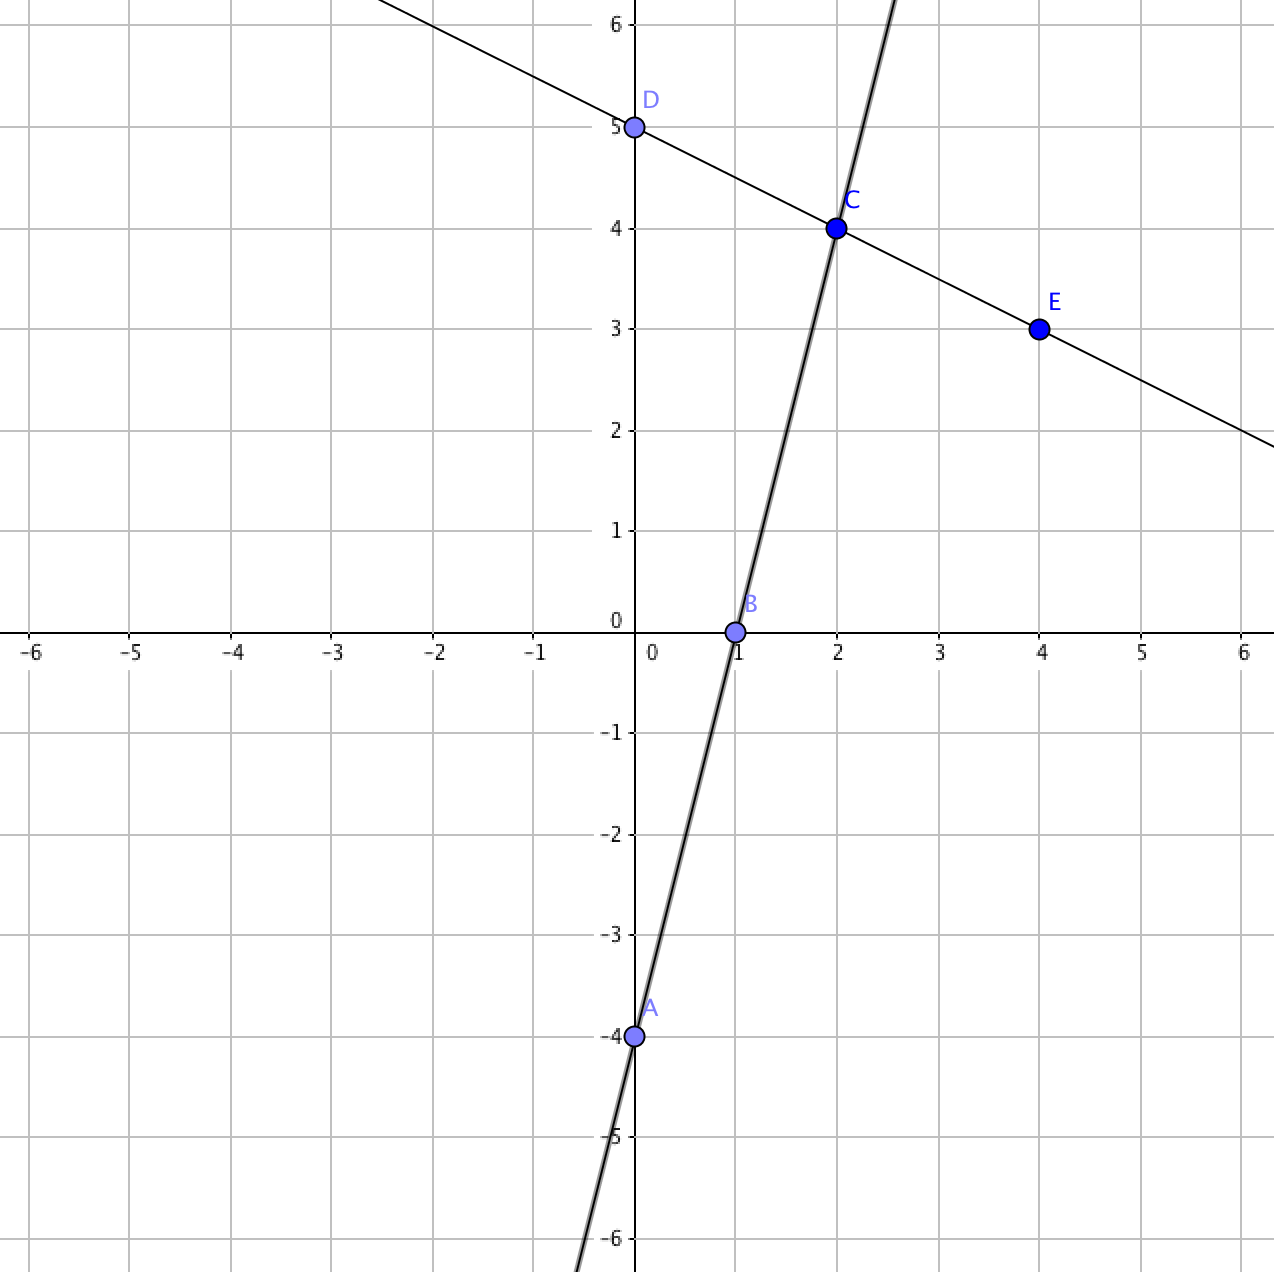
\includegraphics[scale=.35]{intersection.png}	
\end{center}

We can then see that the lines intersect at the point $(2,4)$.  This means that $(2,4)$ is in the solution set to both equations, and is thereby the solution to this system of equations.
\end{example}

This is a useful tool for finding solutions to systems of linear equations as long as being close is good enough.  Unfortunately, some systems of linear equations have solutions that aren't on the grid-lines for a particular scale.

\begin{prblm}
Consider the following system of linear equations.
$$y = -\frac{1}{2}x + 3$$
$$y = 2x$$

What do you think the intersection is?  What could you do to convince someone who didn't agree?

\vspace{4cm}
\end{prblm}


\section{Substitution}

Although most people aren't accustomed to the idea, there is more than one way to do most things in math.  This is a good thing!  If the only way to find the solution to a system of equations was to graph them and point at it, it would be pretty difficult to solve a lot of these systems.  This is where substitution comes in.  Consider two equations in slope-intercept form.

$$y = 2x + 4$$
$$y = 3x + 2$$



Well, if the right side of the first equation is equal to $y$, and the right side of the second equation is equal to $y$, they must be equal to each other!  This is the driving force of substitution.  If two things have the same value, they're equal to each other.

$$2x + 4 = 3x + 2$$

And this is single linear equation that we can solve.

$$\begin{array}{rcl}
2x + 4 & = & 3x + 2\\
4 & = & x + 2 \\
2 & = & x \end{array}$$

So now we know the solution has an $x$-value of $2$.  Nice.  So what about that $y$-value?  We can plug the $x$-value we just found into one of those equations and find out.  We'll choose the first equation.

$$\begin{array}{rcl}
y & = & 2\times2 + 4\\
y & = & 4 + 4\\
y & = & 8 \end{array}$$

Awesome.  Now we think the solution has an $x$-value of $2$, and a $y$-value of $8$.  If this is true, then $(2,8)$ must be a solution to the second equation as well.  We can check that.

$$\begin{array}{rcl}
y & = & 3x + 2 \\
8 & = & 3\times 2 + 2\\
8 & = & 6 + 2 \end{array}$$

Everything checks out.  We've found a solution to this linear system.

\pagebreak

For this last problem, the solution had nice, clean integer values for the solution.  The equations were also given in slope-intercept form.  This won't always be the case.

\begin{example}
Solve the system of linear equations.

$$\begin{array}{rcl}
4y - 16x & = & 25 \\
2y + x & = & -1 \end{array}$$

To use the substitution strategy the way we did last time, we want to solve each equation for either $y$ or $x$.  We had the equations solved for $y$ last time, and solving for $y$ should be natural to us by now, so we'll do that for now.

For the first equation:

$$\begin{array}{rcl}
4y - 16x & = & 25 \\
4y & = & 16x + 25 \\
y & = & 4x + \frac{25}{4} \end{array}$$

And for the second equation:

$$\begin{array}{rcl}
2y + x & = & -1 \\
2y & = & -x -1 \\
y & = & -\frac{1}{2}x - \frac{1}{2} \end{array}$$

Now we're in a similar position as we were at the beginning of the last problem.  We realize that both $-\frac{1}{2}x - \frac{1}{2}$ and $4x + \frac{25}{4}$ are equal to $y$, and so we set them equal to each other.

$$\begin{array}{rcl}
-\frac{1}{2}x - \frac{1}{2} & = & 4x + \frac{25}{4}\\ \\
-\frac{1}{2} & = & 4\frac{1}{2}x + \frac{25}{4}\\ \\
-\frac{1}{2} - \frac{25}{4} & = & 4\frac{1}{2}x\\ \\
-\frac{2}{4} - \frac{25}{4} & = & \frac{9}{2}x\\ \\
-\frac{27}{4} & = & \frac{9}{2}x\\ \\
-\frac{27}{4} \div \frac{9}{2}& = & x \\ \\
-\frac{3}{2} & = & x\\
\end{array}$$

So we've figured out that the solution has an $x$-value of $-\frac{3}{2}$.  Now we need to figure out the $y$-value.  Again, we plug our $x$-value into one of the equations, and the $y$-value should come out.  The great part is that, for the whole sequence where we solved for $y$ in the first equation, each of those equations is equivalent.  We can choose the new version of the first equation to find our $y$-value.

$$\begin{array}{rcl}
y & = & 4\times \left(-\frac{3}{2}\right) + \frac{25}{4}\\
y & = & -\frac{12}{2} + \frac{25}{4}\\
y & = & -\frac{24}{4} + \frac{25}{4}\\
y & = & \frac{1}{4}\\
\end{array}$$

This tells us that the point in the first equation where the $x$-value is $-\frac{3}{2}$ has a $y$-value of $\frac{1}{4}$.  Then, the solution is the point, $\left(-\frac{3}{2}, \frac{1}{4}\right)$.
\end{example}

Let's try a tougher one.

\begin{example}
Solve the system of linear equations.
$$2y - 3x = 9$$
$$5y + 2x = -10$$

For the first equation:

$$\begin{array}{rcl}
2y - 3x & = & 9\\
2y & = & 3x + 9\\
y & = & \frac{3}{2}x + \frac{9}{2} \end{array}$$

And for the second equation:

$$\begin{array}{rcl}
5y + 2x & = & -10\\
5y & = & -10 - 2x\\
y & = & -\frac{2}{5}x - 2 \end{array}$$

Now, setting the right side of each equation equal, 

$$\begin{array}{rcl}
\frac{3}{2}x + \frac{9}{2} & = & -\frac{2}{5}x - 2\\ \\
\frac{3}{2}x + \frac{2}{5}x + \frac{9}{2} & = & - 2\\ \\
\frac{3}{2}x + \frac{2}{5}x & = & -\frac{9}{2} - 2\\ \\
\frac{15}{10}x + \frac{4}{10}x & = & -\frac{9}{2} - \frac{4}{2}\\ \\
\frac{19}{10}x & = & -\frac{13}{2}\\ \\
x & = & -\frac{13}{2} \div \frac{19}{10}\\ \\
x & = & -\frac{65}{19} \\
\end{array}$$
\end{example}


\section{Elimination}

There's yet another strategy for solving systems of linear equations.  This strategy is based on a similar idea as the one the substitution strategy is based on.  Both sides of an equation are equal, and can be replaced with the other.  Consider the following linear system.

$$\begin{array}{rcl}
y - x & = & 4 \\
y + x & = & 2\end{array}$$

From the second unit, we learned that, as long as we add the same thing to both sides, the equation will still be equivalent.  For this strategy, we want to take advantage of the fact that each side of the first equation has the same value.  If we think of the equations as balanced scales, we can think of our next step as taking everything off of the second scale and putting it on the appropriate sides of the first scale.

$$\begin{array}{rcl}
y - x & = & 4 \\
y - x + (y + x) & = & 4 + (2)
\end{array}$$

The stuff in parentheses comes from the second equation.  At this point, we just want to simplify and see what happens.

$$\begin{array}{rcl}
y - x + (y + x) & = & 4 + (2)\\
y - x + y + x & = & 6\\
2y + 0x & = & 6\\
2y = 6
y = 3 \end{array}$$

What happened?

When we took everything from the second equation and put it on the first, we ended up with an equation that has a solution where both of our previous equations had solutions.  Since this value only has a $y$-value and no $x$-value, we have the beginning of a solution!  Let's put that $y$-value in and see what $x$ is.

$$
\begin{array}{rcl}
y - x & = & 4 \\
3 - x & = & 4 \\
3 & = & 4 + x \\
-1 & = & x \end{array}$$

With a value $y$ and $x$, we have a complete solution.  We call this the Elimination Method because the hope is that, when we add the equations together, one of the variables will cancel or be eliminated, leaving us with a linear equation with only one variable.  This worked out for us this time because one equation had a positive $x$, and the other equation had a negative $x$.  If we have more $x$'s in one equation than the other, we'll have some positive or negative $x$'s left over.  In order to make them cancel, we sometimes have to find an equivalent equation.

\begin{example}
Solve the following linear system using the elimination method.

$$\begin{array}{rcl}
y + 2x & = & -2\\
-2y - x & = & 3 \end{array}$$

If we take the second equation and add it to the first equation now, we'll still have an equation with two variables.

$$\begin{array}{rcl}
y + 2x + (-2y - x) & = & -2 + (3)\\
y + 2x - 2y - x & = & 1\\
-y + x & = & 1 \end{array}$$

Like before, we ended up with an equation that has a solution where both of our previous equations had solutions. Unfortunately, it still has two variables, so we can't make any conclusions about it yet.  Let's take a look at the first two equations again.  Notice that the second equation has only one negative $x$, while the first equation has two.  We want to take advantage of equivalent equations.  If we want an equation equivalent to the second equation, but which has two negative $x$'s, we can multiply both sides by 2. Then, the system

$$\begin{array}{rcl}
y + 2x & = & -2\\
-2y - x & = & 3 \end{array}$$

becomes

$$\begin{array}{rcl}
y + 2x & = & -2\\
-4y - 2x & = & 6 \end{array}$$

Because the equations we have are equivalent to the previous equations, the linear system is also equivalent; it will have all of the same solutions.  Let's try adding the equations again.

$$\begin{array}{rcl}
y + 2x + (-4y - 2x) & = & -2 + (6) \\
y + 2x -4y -2x & = & 4 \\
-3y & = & 4 \\
y & = & -\frac{4}{3}
\end{array}$$

Perfect.  We eliminated one of the variables according to plan.  We know that our solution has a $y$-value of $-\frac{4}{3}$.  We can work on finding $x$ now.  This will be easier if we start with the second equation, so we don't have to divide at the end.

$$\begin{array}{rcl}
-2y - x & = & 3 \\
-2\times \left(-\frac{4}{3}\right) - x & = & 3 \\
\frac{8}{3} - x & = & 3 \\
\frac{8}{3} & = & 3 + x \\
\frac{8}{3} - 3 & = & x \\
\frac{8}{3} - \frac{9}{3} & = & x \\
-\frac{1}{3} & = & x \end{array}$$

With values for $x$ and $y$, we can now say that we have a solution.
\end{example}

We're going to do one more example, but there's going to be a twist to it.

\begin{example}
Solve the system of linear equations.

$$\begin{array}{c}
y = \frac{3}{5}x - 6\\
3y + 2x = 1 \end{array}$$

The first thin we have to watch out for is the equals sign.  Remember that the strategy only works because we're taking everything off of one scale and putting it on the appropriate sides of the other scale.  We can't add straight down because the equals signs don't line up.  We have to make sure they do.

$$\begin{array}{rcl}
y & = & \frac{3}{5}x - 6\\
3y + 2x & = & 1 \end{array}$$

That's better.  Now we can clearly see that we need to move the $\frac{3}{5}x$ term to the other side of the first equation.

$$\begin{array}{rcl}
y - \frac{3}{5}x & = & -6\\
3y + 2x & = & 1 \end{array}$$

Now we're in a weird spot.  It looks like we would have to multiply one of the equations by a fraction in order to get the $x$'s to cancel.  Finding that fraction can sometimes take valuable time.  What we're going to do is take advantage of equivalent equations again, and we're going to fix both of the equations.  We'll look at the coefficient of the $x$ in the first equation, and multiply the second equation by it.  Then we'll look at the coefficient of $x$ in the second equation and multiple by first equation by it.  This way, the $x$'s in both equations will be multiplied by both coefficients, and this should make them cancel.


$$\begin{array}{rcl}
y - \frac{3}{5}x & = & -6\\
3y + 2x & = & 1\\ \\
y - \frac{3}{5}x & = & -6\\
\frac{3}{5}\times 3y + \frac{3}{5}\times 2x & = & \frac{3}{5}\times 1\\ \\
y - \frac{3}{5}x & = & -6\\
\frac{9}{5}y + \frac{6}{5}x & = & \frac{3}{5}\\ \\
2y - 2\times \frac{3}{5}x & = & 2\times (-6)\\
\frac{9}{5}y + \frac{6}{5}x & = & \frac{3}{5}\\ \\
2y - \frac{6}{5}x & = & -12 \\
\frac{9}{5}y + \frac{6}{5}x & = & \frac{3}{5} \end{array}$$

And now, when we add the equations together, the $x$'s will cancel.

$$\begin{array}{rcl}
2y - \frac{6}{5}x + (\frac{9}{5}y + \frac{6}{5}x) & = & -12 + (\frac{3}{5}) \\
2y - \frac{6}{5}x + \frac{9}{5}y + \frac{6}{5}x & = & -\frac{60}{5} + \frac{3}{5} \\
2y + \frac{9}{5}y & = & -\frac{57}{5} \\
\frac{10}{5}y + \frac{9}{5}y & = & -\frac{57}{5} \\
\frac{19}{5}y & = & -\frac{57}{5} \\
y & = & -\frac{57}{5} \div \frac{19}{5}\\
y & = & -3
\end{array}$$

We have a $y$-value.  What's missing?

$$\begin{array}{rcl}
3y + 2x & = & 1\\
3 \times -3 + 2x & = & 1 \\
2x & = & 10 \\
x & = & 5 \end{array}$$

This tells us that our solution is $(5,-3)$.
\end{example}

As we can see, some problems are more well-suited for elimination than others.

\pagebreak

\section*{Exercises}

\begin{exercise}
Find the slope of the line that goes through (0,6) and (2,0)
\end{exercise}

\bigskip

\begin{exercise}
Find the slope of the line that goes through (0,2) and (6,0)
\end{exercise}

\bigskip

\begin{exercise}
	Find the solution for the following linear system:
	$$
	\begin{array}{rcl}
	x & = & 4 \\
	y & = & 2x+1	
	\end{array}
	$$
	Is there one method for solving this system that is easier than the others? Give evidence for your answer. 
\end{exercise}
\bigskip

\begin{exercise}
	Find a linear system that has the solution $(2,5)$.
\end{exercise}
\bigskip

\begin{exercise}
Your philosophy teacher wants you to compare apples and oranges for an assignment. Your friend picks up a total of 12 bundles of fruit and paid \$74.00. The apples weighed 5 lbs per bundle and the oranges weighed 4 lbs per bundle. If the bundles of apples cost \$5 a piece and the bundles of oranges cost \$7 a piece, how many bundles of apples did your friend buy?
\end{exercise}
\bigskip

\begin{exercise}
Consider the linear system:
$$
\begin{array}{rcc}
y& = & x \\
y & = & -x 	
\end{array}
$$
with respective slopes 1 and -1. If we change the slopes of the two lines to 2 and -2, without changing the y-intercept, does it change the solution? If so, what is the new solution. Provide evidence for your claim. 	
\end{exercise}

\bigskip

\begin{exercise}
Solve the following system of equations using whatever method you choose:
$$
2x-y = 3
$$
$$
-3y = 4 +x
$$	
\end{exercise}

\bigskip

\begin{exercise}
	In what type of situations is it more difficult to use graphing than substitution or elimination to solve a linear system? Give an example of a system in which this is true. 
\end{exercise}

\bigskip

\begin{exercise}
Find the solution for the system:
$$
\begin{array}{rcl}
7x + 4y & = & 3 \\
x + \frac{1}{7}y & = & 3	
\end{array}
$$
\end{exercise}
\bigskip

\begin{exercise}
Solve the following system in two ways (using substitution and elimination) and compare your answers:
$$
\frac{1}{2}x + y = 6
$$	
$$
4x =y
$$

Should the solutions be the same or different. Provide evidence for your answer.
\end{exercise}

\bigskip

\begin{exercise}
It costs \$5.00 for a student and \$10.00 for non-students to see a movie at the Cinema 12. If the theater had 75 people go to a movie one night and made \$500 dollars from ticket sales, how many students saw a movie that night?
\end{exercise}

\bigskip

\begin{exercise}
	Find the solution for the linear system:
	$$
	2x+y=17
	$$
	$$
	\frac{1}{2}y=-x +1
	$$	
\end{exercise}

\bigskip

\begin{exercise}
Use whatever method you choose to find the solution for the system:
$$
\begin{array}{rcl}	
1002x + 404y &=  & 2016 \\ \\
4x + 6y &= &36
\end{array}
$$ 
\end{exercise}
\bigskip

\begin{exercise}
Solve the following linear system:
$$
2x+ y = 7 
$$
$$
\frac{1}{3}y = -\frac{2}{3}x + \frac{7}{3}
$$	
\end{exercise}

\bigskip

\begin{exercise}
Find a point on the line, and write it in point-slope form using the chosen point.
\end{exercise}

\bigskip

\begin{exercise}
Find the slope-intercept form of a line passing through the points (-1,-1) and (7,3).
\end{exercise}

\bigskip

\begin{exercise}
Choose three different slopes, and find the y-intercepts of  the lines with those slopes passing through the point (2,2).  Graph these lines on the same graph.
\end{exercise}

\bigskip

\begin{exercise}
	Consider the function $16y + 10 + x = 2x + 42$. Is this function linear? How can we tell?
\end{exercise}


\chapter{Quadratics}

While understanding how to work with lines is incredibly useful for modeling many relationships, we know that the real world is a bit more complex.  When we look at the growth of a population over time or at the path that a ball takes through the air, we quickly realize that linear equations can only do so much.  One of the first step forward is to begin dealing with functions and equations that involve higher exponents.  

This chapter is going to be about equations that are the product of two linear terms.  That is, rather than dealing with functions like $f(x) = 3x - 1$ or $f(x) = \frac{1}{4}x + 2$, we'll be dealing with things like these multiplied together, or $f(x) = (3x-1)(\frac{1}{4}x + 2)$.  We'll cover the different forms that these equations can take, and we'll cover the ways we can solve for our inputs.

\begin{presentation}
\begin{defn}
Polynomial

An expression which can be written as the product of linear expressions.  These expressions may require complex numbers.
\end{defn}
\end{presentation}

\begin{defn}
Quadratic

A polynomial which is the product of exactly two linear expressions.
\end{defn}

The simplest quadratic we deal with is the function which simply squares inputs.  If we put in a 3, we get out a 9.  If we put in a 4, we get out a 16.  We will call this the squaring function.  Unlike the doubling function, the squaring function is not linear.  It can be written as $f(x) = x^2$.  Note that $x$ is a linear expression.  This means $x^2$ is the product of two linear expressions, so it conforms to our definition of quadratic.

\begin{example}
If we want to find the area of a rectangle, we multiply the length by the width, $A = lw$.  If we have 10 feet of wood, we can express the area as a function of the length.  Because we have 10 feet of wood to make two lengths and two widths, we know $2l + 2w = 10$.   If we solve one for $w$, we can replace the $w$ in the area equation by substituting.

$$\begin{array}{rl}
2l + 2w & = 10\\
2w & = 10 - 2l\\
w & = 5 - l\end{array}$$

Then the area is the product of two linear expressions containing $l$, 

$$A(l) = l*(5 - l)$$
\end{example}

\section*{Forms of Quadratics}

\subsection*{Factored Form}

If a quadratic is expressed as the product of two linear pieces, we say that it is in factored form.

\begin{defn} Factor

One of the linear terms that is multiplied in the factored form of a polynomial.
\end{defn}


\begin{presentation}
\begin{defn} Root
The roots of a polynomial are the inputs for which it gives an output of zero.  If we graph the polynomial, the roots will show up as $x$-intercepts.  When a quadratic is in factored form, it is easy to identify its roots, since only one factor needs to be zero for the whole polynomial to be zero.
\end{defn}
\end{presentation}

\begin{presentation}
\begin{example}
To find the roots of the quadratic $(x-2)(x+4)$, we need to find where it is equal to zero.  It can only be zero if either $(x-2)$ or $(x+4)$ is equal to zero.  Then the roots correspond to the $x$-intercepts of the linear functions made by each output.

To find the first root, we find out where $(x-2) = 0$.  This is a simple linear equation, and we know that it is true if $x = 2$.

To find the second root, we similarly find out where $(x+4) = 0$.  Here, we know that it is true if $x = -4$.

Since either one of these factors giving an output of zero will make the output of the quadratic zero, both of the solutions we found are roots of the quadratic.

\end{example}
\end{presentation}

It is important to mention that not every quadratic can be expressed in factored form using only real numbers.  Real numbers have an unfortunate name in that they are not any more real than complex numbers, which have an `imaginary' part.  We won't worry too much about complex numbers in this class.  If a quadratic cannot be expressed in factored form in real numbers, we can still express it in other ways.

\subsection*{Standard Form}

The `standard form' of a quadratic expression is as the sum of terms with different exponents.  $3x^2 + 6x - 9$ is an example of this.  It is equivalent to $3(x + 3)(x - 1)$.

While we can't write every quadratic in factored form (yet), we can always express them in standard form.  $x^2 +x+ 1$ is a quadratic which doesn't have a factored form that we can use, here.

\begin{prblm}
Why doesn't $x^2 +x + 1$ have a factored form?
\end{prblm}

\subsection*{Vertex Form}

This form of a quadratic is most closely related to the point-slope form of a line.  Just as with linear functions, switching between the various forms of quadratics can give you different pieces of important information.

\begin{defn} Vertex

A vertex is the lowermost or uppermost point of a parabola.
\end{defn}

To understand vertex form, we first elaborate on the simplest quadratic: $x^2$.  Its vertex will be at the point $(0,0)$.  However, by moving this simple function, called a `parent function', we can make quadratics with vertices at other points.  We call it the parent function because...

When thinking about every point as $(x, f(x))$, if we want to move the vertex to the left or the right, we change the $x$-value.  If we want to move the vertex up or down, we change the $f(x)$ value.  Thus, any point where the graph has been moved to the right by $h$ and up by $k$ will be $(x + h, f(x) + k)$.  However, we only want our inputs to be $x$'s, so, adjusting all $x$'s appropriately, $(x, f(x-h)+k)$

If we also allow the graph to be stretched, we can easily account for this in vertex form.  $$a(x-h)^2 + k$$

\begin{example}

We want to find a quadratic with its vertex at the point $(1,2)$.

First, we look at the parent function, $f(x) = x^2$.  If all points on it are expressed $(x, f(x))$, the vertex is normally at $(0,0)$.  If we want the vertex to be at $(1,2)$, we have to move over one, and up by two.  Thus, our new points will be $(x, f(x-h)+k)$, making our new function $g(x) = (x-1)^2 + 2$.

This is then a quadratic with a vertex at the point $(1,2)$.

\end{example}

\begin{prblm}
If we know the factored form of a quadratic, how can we find the vertex form?
\end{prblm}

\section*{Manipulating Quadratics}

Now that we've covered the forms for quadratic expressions, we need a way to switch between them.  If we are solving a problem where we need to know the roots of the quadratic, we would prefer it in factored form.  If we are solving a problem where we need to know where the maximum value occurs, we would prefer it in vertex form.  If we are solving a problem where we are finding where two quadratics intersect, we would prefer it in standard form.

\subsection*{More Fun With the Distributive Property}

One of the most important properties that we regularly use in algebra is the Distributive property.  In the following case, the 3 gets multiplied by each term in parentheses.

$$3(x-4) = 3x - 12$$

In this case, the -6 gets multiplied by each term in the parentheses, but some simplification is required.

$$\begin{array}{rl}
-6(\frac{1}{4}- x) & = \\ & \\
-6\frac{1}{4} -(-6x) & = \\ & \\
-\frac{3}{2} + 6x\end{array}$$

In both of these examples, only a constant was being distributed, but the distributive property works no matter what we're multiplying.  Most importantly, it works with groups of parentheses.

\begin{example}

In the following group, the entire factor $(2x + 3)$ gets multiplied by each term in the other factor.
$$(2x + 3)(5-x) = (2x+3)5 - (2x+3)x$$

From here, we have two more terms, and each of these can be simplified by distributing.

$$\begin{array}{rcll}
(2x + 3)5 & - & (2x + 3)x & = \\
10x+15 & - & 2xx+3x & = -2x^2 + 13x + 15\end{array}$$
\end{example}

After reordering the terms from highest exponent to lowest, we recognize this as a quadratic in standard form.

\begin{example}
Put the following expression into standard form.

$$(x + \frac{1}{2})^2$$

First, we want to write this as a product.  Then we can comfortably distribute.

$$\begin{array}{rl}
(x+\frac{1}{2})^2 & = (x+\frac{1}{2})(x+\frac{1}{2}) \\ & \\
& = x(x+\frac{1}{2})+ \frac{1}{2}(x+\frac{1}{2}) \\ & \\
& = x^2 + \frac{1}{2}x + \frac{1}{2}x + \frac{1}{2}\frac{1}{2} \\ & \\
& = x^2 + x + \frac{1}{4}
\end{array}$$
\end{example}

\subsection*{Factoring Quadratics}

If you're looking at a quadratic in standard form, but if you want to know the roots, it is very useful to put it into factored form.  We do this by considering what linear terms we would have to distribute in order to achieve a particular standard form.

\begin{example}

When we look at the following quadratic in standard form, we take note of a few things.

$x^2 + 5x + 6$

First, if we were to write it as $(x + a)(x + b)$, we know that $a$ and $b$ would have to multiply together to give 6.  We also know that $ax + bx = 5x$.  So now our job is to figure out what $a$ and $b$ are.  We can start by listing everything that we can that will multiply to get 6.

1 and 6

2 and 3

If we add 1 and 6, we get 7.  If we add 2 and 3, we get 5.  Since we needed $a$ and $b$ to add up to 5, we know that our factored form is $(x + 2)(x + 3)$.  We can always check this by distributing. 

\end{example}

\begin{example}

If we want to factor $x^2 +x - 6$, we have something new to consider.  We need numbers which will multiply to give us 6, but now we can use either positive or negative numbers.

1 and -6

-1 and 6

2 and -3

-2 and 3

Since $x$ has a coefficient of +1, here, we can see that the factored form must be $(x+3)(x + -2)$.  We then simplify this to $(x+3)(x - 2)$

\end{example}

\section*{Completing the Square}

Any quadratic expression can be expressed in vertex form.  However, since we haven't reached how to express every quadratic in factored form, the previously discussed strategy isn't sufficient for every situation.  However, if we are given a quadratic in standard form, we can always put it in vertex form.

First, we should convert from vertex form to standard form.

$$\begin{array}{rcl}
a(x-h)^2 + k & = & a(x^2 - 2hx + h^2) + k\\
& = & ax^2 - 2ahx + ah^2 + k\end{array}$$

If we look long and hard enough at this alphabet soup, we notice that only the first two terms have $x$ in them.  Each of those terms also has $a$, meaning that we have enough information to sort out what $h$ has to be by identifying $a$ and then looking at the term with $x^1$.

\begin{example}
Where is the vertex of this quadratic?
$$3x^2 - 4x + 2$$

First, we ask where the $x$-value of the vertex is.  Notice that $a = 3$.  Also, $-2ahx$ corresponds to $-4x$.  Setting these equal,
$$\begin{array}{rcl}
-2ahx & = & -4x \\
-6hx & = &-4x \\
hx & = & \frac{2}{3}x \\
h & = & \frac{2}{3}
\end{array}$$

Now, if we want to figure out the $y$-value of the vertex, we need to look at what we have so far.

$$3(x - \frac{2}{3})^2 + k$$

When we try to put this back into standard form, we have

$$\begin{array}{rcl}
3(x - \frac{2}{3})^2 + k & = & 3(x - \frac{2}{3})(x - \frac{2}{3})+ k\\& & \\
& = & (3x - 2)(x - \frac{2}{3}) + k\\& & \\
& = & 3x(x - \frac{2}{3}) - 2(x - \frac{2}{3}) + k \\& & \\
& = & 3x^2 - 2x - 2x + \frac{4}{3}) + k \\ & & \\
& = & 3x - 4x + \frac{4}{3} + k
\end{array}$$

Since our original expression has a constant term of 2, we need $\frac{4}{3} + k = 2$.  Thus, $k = \frac{2}{3}$

We then know $h$ and $k$, so our vertex is at $(\frac{2}{3}, \frac{2}{3})$.

\end{example}

\section*{Solving Quadratic Equations}

A quadratic equation is any equation with a quadratic expression in it.  Sounds reasonable enough!

\begin{example}
$x^2 - 2x + 1 = 4$ is a quadratic equation.  By graphing the quadratic expression, we can see that it equals 4 when $x = -1$ and when $x = 3$.
\end{example}

This is a rather crude way to see the solutions, so we want to use algebra if we can.  We can do this with either factoring or putting the expression in vertex form.  The latter is the most consistently successful method, but we will begin by demonstrating factoring.

We want to find solutions to the following equation,

$$x^2 - 3x - 4 = - 6$$

A common mistake is to factor this expression without a goal in mind.  The reason factoring a quadratic is useful is because it is easy to find where the expression equals zero.  If we factor the left side of the equation now, we would have to figure out where it equals -6, which is not nearly so easy.  Before factoring, we should make sure the right side is zero so that we get the information we want.

$$x^2 - 3x + 2 = 0$$

We have a new quadratic expression on the left side, and if it were in factored form, it would then be easy to find solutions for $x$.  Now we need two numbers we can multiply to get 2, but add to get -3.  Since -1 and -2 are the only valid choices, we can change to the factored form.

$$(x-1)(x-2) = 0$$

And we know this will only be true when $x = 1$ or $x = 2$, so 1 and 2 are our solutions to this quadratic equation.

\begin{example}
Solve the quadratic equation by factoring.
$$(x - 5)(x + 1) = -8$$

You may have noticed: the quadratic expression is already factored.  However, the factored form being equal to -8 isn't the simplest to find.  We need a different expression that's equal to zero before factoring gets us anything useful.  We'll put it into standard form first and see where that gets us.

$$\begin{array}{rcl}
(x - 5)(x + 1) & = & -8 \\
x(x+1) - 5(x+1) & = & -8 \\
x^2 + x - 5x - 5 & = & -8 \\
x^2 - 4x - 5 & = & -8
\end{array}$$

Great!  Now that we're here, we can do what we did last time.  We need a quadratic expression equal to zero, and then we can factor it and get information that helps us.

$$\begin{array}{rcl}
x^2 - 4x - 5 & = & -8 \\
x^2 - 4x + 3 & = & 0 \\
(x - 1)(x - 3) & = & 0 \\
\end{array}$$

Now we can clearly see that our solutions are 1 and 3.

\end{example}

If we need to find a solution with a quadratic in vertex form, we want to solve for the squared expression first, and then we can worry about $x$.

If we have
$$\frac{1}{4}(x - 1)^2 - 4 = 0$$

We want to use inverse operations to undo everything that's been done to the $x$, in the reverse order.

$$\begin{array}{rcl}
\frac{1}{4}(x - 1)^2 - 4 & =& 0\\
\frac{1}{4}(x - 1)^2 & =& 4 \\
(x - 1)^2 & =& 16 \\
x - 1 & =& 4 \text{ or } -4\\
x & = & 5 \text{ or } -3\\
\end{array}$$

Thus, we have 5 and -3 as solutions.  Because we don't want a bunch of `or's in our equations, there's a symbol for representing positive or negative values: $\pm$.  $\pm4$ means either +4 or -4.  It's important to remember that, when taking the square root of an expression, the result can be either positive or negative.

\begin{example}
Find solutions to
$$x^2 - 10x + 10 = 0$$

First, we find the vertex.  We know that whatever $h$ is will give us the term $-10x$ when we distribute $(x - h)^2$, so $h = 5$.  Now, to find $k$, 

$$\begin{array}{rcl}
x^2 - 10x + 10  & = & (x - 5)^2 + k\\
x^2 - 10x + 10  & = & x^2 - 10x + 25 + k \\ 
10  & = & 25 + k \\ 
-15  & = & k
\end{array}$$

Now that we know what the vertex form of this quadratic will look like, we can begin solving for $x$.

$$\begin{array}{rcl}
(x - 5)^2 - 15 & = & 0 \\
(x - 5)^2 & = & 15 \\
x - 5 & = & \pm \sqrt{15} \\
x & = & \pm \sqrt{15} + 5\\
\end{array}$$

Since 15 is not a perfect square, we usually leave our answers in this form since it is more exact.  We could also find decimal approximations, but they are more difficult to work with since we won't be able to go backward.  We write our solutions as a list as usual:

$5 + \sqrt{15}$, 

$5 - \sqrt{15}$

\end{example}
%\section*{Exercises}

\begin{exercise}
	Find the solution for the following linear system:
	$$
	\begin{array}{rcl}
	x & = & 4 \\
	y & = & 2x+1	
	\end{array}
	$$
	Is there one method for solving this system that is easier than the others? Give evidence for your answer. 
\end{exercise}
\bigskip

\begin{exercise}
	Find a linear system that has the solution $(2,5)$.
\end{exercise}
\bigskip

\begin{exercise}
Your philosophy teacher wants you to compare apples and oranges for an assignment. Your friend picks up a total of 12 bundles of fruit and paid \$74.00. The apples weighed 5 lbs per bundle and the oranges weighed 4 lbs per bundle. If the bundles of apples cost \$5 a piece and the bundles of oranges cost \$7 a piece, how many bundles of apples did your friend buy?
\end{exercise}

\begin{exercise}
Consider the linear system:
$$
\begin{array}{rcc}
y& = & x \\
y & = & -x 	
\end{array}
$$
with respective slopes 1 and -1. If we change the slopes of the two lines to 2 and -2, without changing the y-intercept, does it change the solution? If so, what is the new solution. Provide evidence for your claim. 	
\end{exercise}

\bigskip

\begin{exercise}
Solve the following system of equations using whatever method you choose:
$$
2x-y = 3
$$
$$
-3y = 4 +x
$$	
\end{exercise}

\bigskip

\begin{exercise}
	In what type of situations is it more difficult to use graphing than substitution or elimination to solve a linear system? Give an example of a system in which this is true. 
\end{exercise}

\bigskip

\begin{exercise}
Find the solution for the system:
$$
\begin{array}{rcl}
7x + 4y & = & 3 \\
x + \frac{1}{7}y & = & 3	
\end{array}
$$
\end{exercise}
\bigskip

\begin{exercise}
Solve the following system in two ways (using substitution and elimination) and compare your answers:
$$
\frac{1}{2}x + y = 6
$$	
$$
4x =y
$$

Should the solutions be the same or different. Provide evidence for your answer.
\end{exercise}

\bigskip

\begin{exercise}
It costs \$5.00 for a student and \$10.00 for non-students to see a movie at the Cinema 12. If the theater had 75 people go to a movie one night and made \$500 dollars from ticket sales, how many students saw a movie that night?
\end{exercise}

\bigskip

\begin{exercise}
	Find the solution for the linear system:
	$$
	2x+y=17
	$$
	$$
	\frac{1}{2}y=-x +1
	$$	
\end{exercise}

\begin{exercise}
Use whatever method you choose to find the solution for the system:
$$
\begin{array}{rcl}	
1002x + 404y &=  & 2016 \\ \\
4x + 6y &= &36
\end{array}
$$ 
\end{exercise}

\begin{exercise}
Solve the following linear system:
$$
2x+ y = 7 
$$
$$
\frac{1}{3}y = -\frac{2}{3}x + \frac{7}{3}
$$	
\end{exercise}



\chapter{Rational Expressions}

If we view the last chapter as an introduction to the multiplication of linear expressions, we can look at this chapter as the equivalent introduction for division. Therefore, it may be helpful to review what a rational number is. Hence, a rational number is to integers as a rational expression is to linear expressions.

\begin{defn}[Rational Expression]
	A rational expression is an expression that can be written as a fraction of polynomials. 
\end{defn}

Rational expressions 

\begin{defn}[Relatively Prime]
	Two numbers (or expressions) are relatively prime if the only factor they have in common is 1. A rational expression is said to be in simplest form if the numerator and denominator are relatively prime. 
\end{defn}

\begin{example}
	Put the following rational expression into simplest form:
	
	\[
	\frac{x^2+2x+1}{x+1}
	\]
	
	What we want to check here is whether the numerator and denominator have any common factors. The expression $x+1$ is already prime. So we have to check the factors of $x^2+2x+1$. When we factor this quadratic, we get $(x+1)(x+1)$. Now we have:
	\[
	\frac{(x+1)(x+1)}{(x+1)}
	\]
	
	Since the numerator and denominator have a common factor, we can divide out the factor ($x+1$) to find:
	\[
	\frac{(x+1)(x+1)}{(x+1)}= \frac{\xcancel{(x+1)}(x+1)}{\xcancel{(x+1)}}=\frac{(x+1)}{1}=x+1
	\]
\end{example}


The benefit from factoring using vertex form is every quadratic with real roots can be factored. However, when dealing with rational expressions, we can usually tell if we need to factor to the point of irrational roots. 

\begin{example}
Consider the following rational expression:

\[
\frac{x^2+3x+7}{(x+\frac{\sqrt{9}-3}{2})}
\]

If we want to put this quadratic into simplest form, we would want to find whether these have any common factors. The denominator is already prime, since it is linear, but the numerator is not. We cannot factor this quadratic ($x^2+3x+7$) easily. But if we look at the denominator, which is prime, we can see that in order to possibly simplify this quadratic, we would need to find that $(x+\frac{\sqrt{9}-3}{2}$ is a factor of $x^2+3x+7$. In this case factoring to the point of irrational roots would be necessary. But situations like this will arise in only a few exercises. 
\end{example}


Thus rational expressions require some degree of critical thinking whether we should factor a polynomial to its linear terms or not. Many times factoring to linear terms will not help us divide out any common factors.

\begin{example}
Simplify to simplest form the following rational expression:

\[
\frac{x^2-9x+20}{x+1}
\]	

If we want to reduce this to its simplest form, we would need to find $(x+1)$ is a factor of $x^2-9x+20$. If we were to factor this, we would find that $x^2-9x+20= (x-4)(x-5)$. Thus we have:
\[
\frac{(x-4)(x-5)}{(x+1)}
\]
Since the numerator or the denominator have no common factors, we know that this must be the simplest form. 
\end{example}

The fun doesn't stop here. Much like with regular fractions, putting these rational expressions into simplest form is just the beginning. We can add, subtract, multiply, and divide these expressions using the same methods we add, subtract, and divide fractions. Let's first explore adding rational expressions.

\begin{example}[Adding Rational Expressions]
Simplify the following:

\[
\frac{x^2}{(x-2)}+\frac{-4}{(x-2)}
\]
When we are adding or subtracting, we need to make sure we have the same denominators for both rational expressions. In this case, we already do. Therefore, we simply add the numerators and keep the denominators the same. 

\[
\frac{x^2}{(x-2)}+\frac{-4}{(x-2)}=\frac{x^2-4}{(x-2)}
\]

But we still aren't done! The directions said to simplify, which means we need to make sure our new rational expression is in simplest form. If we factor the numerator, we find:
\[
\frac{x^2-4}{(x-2)}=\frac{(x-2)(x+2)}{(x-2)}=\frac{\xcancel{(x-2)}(x+2)}{\xcancel{(x-2)}}=x+2
\]
Now we are done. Our answer in simplest form is $x+2$.
\end{example}

Adding and subtracting are easy when we have denominators that are the same, but that isn't always the case. Often, we will have to get common denominators before we can perform the operation. 

\begin{example}[Addition without Common Denominator]
Simplify the following rational expressions:

\[
\frac{x^2+7x+6}{(x+1)}+\frac{2x}{3}
\]	
Bummer. Now we have to make a choice. Do we want to try to simplify either expression before we add? First let's check if we can quickly factor anything. The numerator of the first expression is $x^2+7x+6$, which we can factor into $(x+6)(x+1)$. Therefore, we have:
\[
\frac{(x+6)(x+1)}{(x+1)}+\frac{2x}{3}=\frac{(x+6)\xcancel{(x+1)}}{\xcancel{(x+1)}}+\frac{2x}{3}=\frac{(x+6)}{1}+\frac{2x}{3}
\]
Still not ready to add, because we need these fractions to have the same denominator. So, we can multiply both the numerator and denominator of the first expression by three to get:
\[
\frac{3(x+6)}{3}+ \frac{2x}{3}
\]
Now we are good to go. By adding across, we find:
\[
\frac{3(x+6)+2x}{3}
\]
Last but not least, we want to put this expression in simplest form.
\[
\frac{3(x+6)+2x}{3}=\frac{5x+18}{3}.
\]
\end{example}

Finding a common denominator will not always be as easy as multiplying by an integer. More often than not, we will have to multiply the numerator and denominator by a full expression. In this next example, we have to multiply by $x$.

\begin{example}[Subtraction]
Subtract the following rational expressions. Simplify your answer:
\[
\frac{x-2}{1}-\frac{8}{x}
\]	
Once again, we don't have common denominators. A quick check also tells us that both these expressions are already simplified. Therefore, next step is getting a common denominator.
\[
\frac{x}{x} \cdot \frac{x-2}{1} -\frac{8}{x} = \frac{x^2 -2x}{x}-\frac{8}{x}=\frac{x^2-2x-8}{x}
\]
Can we simplify this? Let's check:
\[
\frac{x^2-2x-8}{x}=\frac{(x-4)(x+2)}{x}
\]
When we factor the numerator, we find that the numerator and denominator have no common factors. Therefore, this is simplified. 
\end{example}





\chapter*{Useful Definitions}


\begin{defn2}[Integer]\label{Integer}
	A number is an integer if it has no fractional part. An integer can be either positive or negative. We denote the set of integers as $\mathbb{Z}$. \\$-4, -2, 0, 3,17,  9002$ are all examples of integers. 
\end{defn2}

\begin{defn2}[Real Number]\label{Real Number}
A real number is a value that can be represented on a number line. We denote the set of all real numbers as $\mathbb{R}$.
\end{defn2}


\begin{defn2}[Imaginary Constant]\label{Imaginary Constant}
	The imaginary constant $i$ is defined as $i= \sqrt{-1}$.
\end{defn2}

\begin{defn2}[Complex Number]\label{Complex Number}
	A complex number is any number of the form $a+bi$ where $a$ and $b$ are real numbers and $i$ is the imaginary constant. 
\end{defn2}

\begin{defn2}[Solution Set]\label{Solution Set}
	A number or set of numbers that a variable could be to make the equation true.  A solution to an equation with multiple variables has a value for each variable. 
\end{defn2}


\begin{defn2}[Distributive Property]\label{Distributive Property}
	The distributive property tells us that $a(b+c)=ab+ac=(b+c)a$. 
	
	\noindent
	\emph{There is a well detailed example \hyperref[Distributive Example]{here}.}
\end{defn2}





\begin{defn2}[Degree]\label{Degree}
The degree of a polynomial is the value of the largest non-negative exponent. 

\noindent
\textbf{Ex.} \emph{The degree of the polynomial $g(x)=x^3 +x-8$ is 3.}
\end{defn2}


\chapter*{Appendix}



\theendnotes

\end{document}
